\documentclass[landscape]{article}
\usepackage[utf8]{inputenc}
\usepackage[T1]{fontenc}
\usepackage[dvipsnames]{xcolor}
\usepackage{tikz}
\usepackage{geometry}
\usepackage{amsmath}
\usepackage{helvet}

\geometry{a1paper, margin=1.5cm}
\renewcommand{\familydefault}{\sfdefault}

% Schalenfarben der Energiedoku
\definecolor{shell2}{RGB}{173, 216, 230} % Mesonen (Blau)
\definecolor{shell3}{RGB}{255, 218, 185} % Quarks (Peach)
\definecolor{shell4}{RGB}{152, 251, 152} % Atome (Grün)
\definecolor{shell5}{RGB}{255, 215, 0}   % Goldene Matrix (Gold)
\definecolor{transuran}{RGB}{255, 105, 180} % Transurane (Pink/Instabil)
\definecolor{background}{RGB}{25, 25, 35}

\begin{document}
	\pagecolor{background}
	\color{white}
	
	\begin{center}
		\fontsize{70}{80}\selectfont \textbf{\#Energiedoku: Das Arithmetische System} \\
		\fontsize{30}{40}\selectfont \textit{Vom Wasserstoff-Vakuum bis zum Neptunium-Horizont} \\
		\vspace{0.8cm}
		\Large \textbf{Modell: Quaternionen-Primzahl-Symmetrie | Standort: Bamberg}
	\end{center}
	
	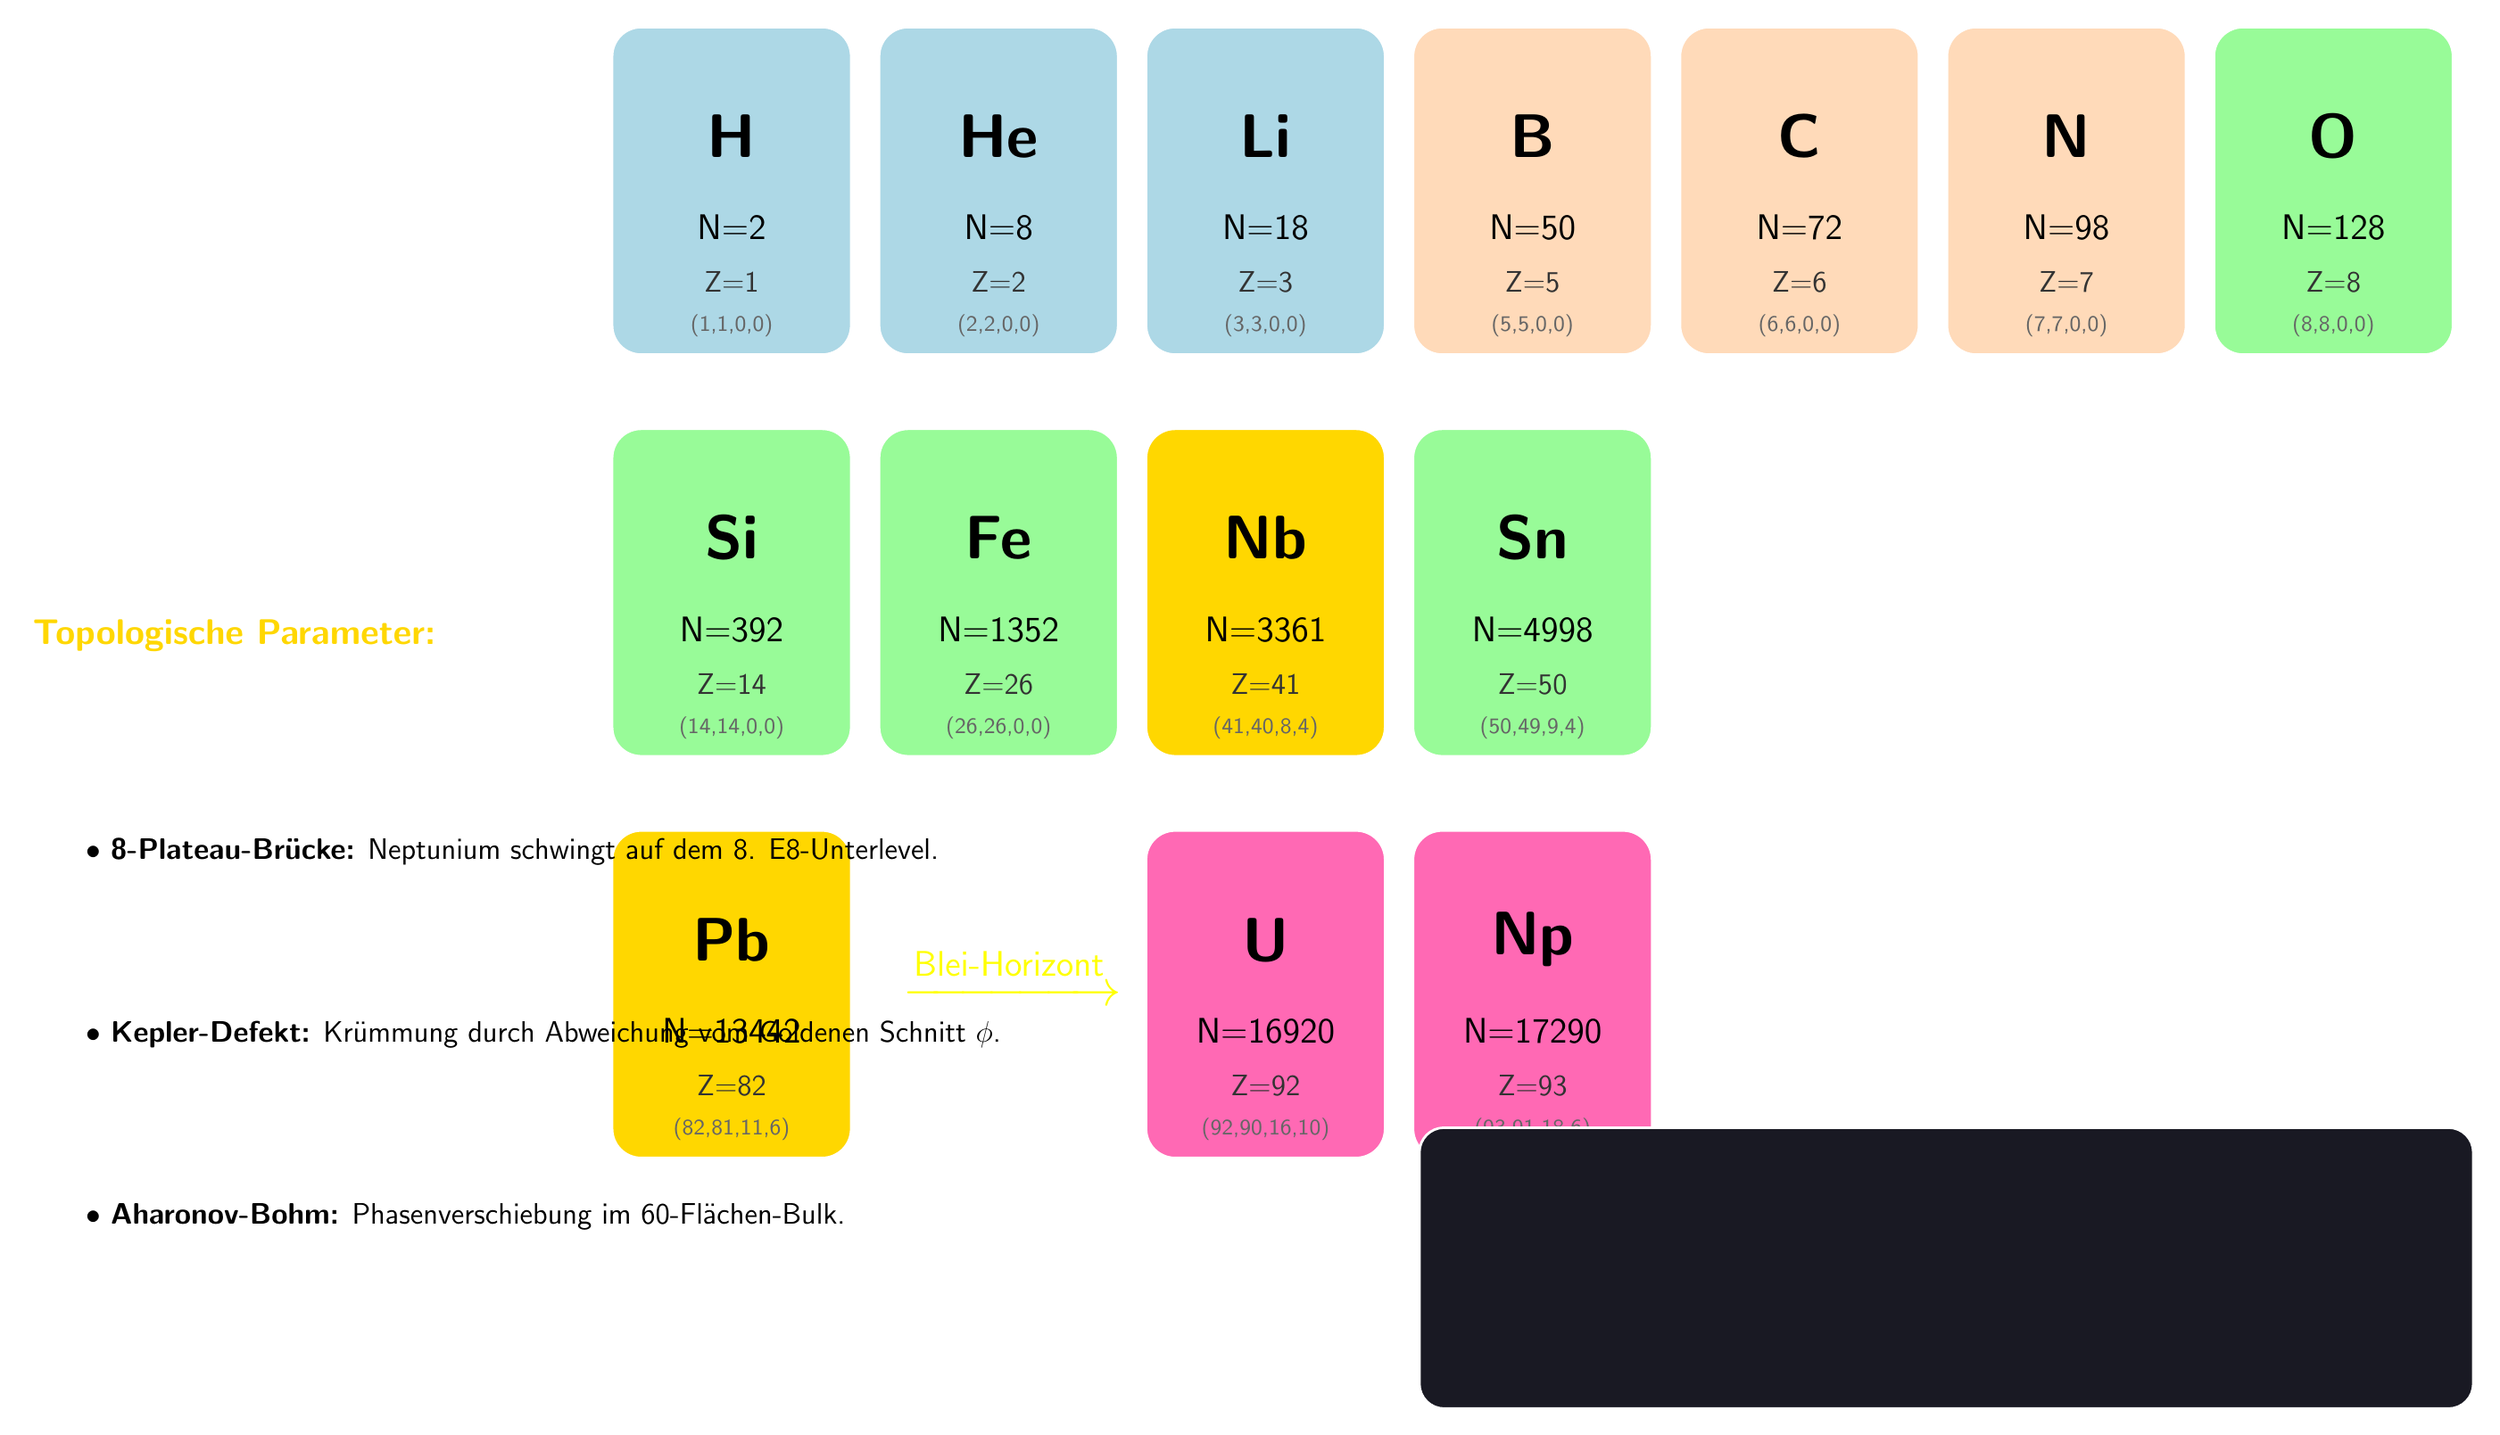
\begin{tikzpicture}[x=3.8cm, y=5.2cm]
		
		% --- HILFSFUNKTION FÜR KACHELN ---
		\newcommand{\boxel}[7]{ % #1:x, #2:y, #3:Sym, #4:N, #5:Z, #6:Konfig, #7:Farbe
			\draw[fill=#7, draw=white, line width=1.5pt, rounded corners=12pt] (#1, #2) rectangle (#1+0.9, #2+0.9);
			\node[anchor=center, font=\fontsize{45}{50}\selectfont, color=black] at (#1+0.45, #2+0.6) {\textbf{#3}};
			\node[anchor=center, font=\Large, color=black] at (#1+0.45, #2+0.35) {N=#4};
			\node[anchor=center, font=\large, color=black!80] at (#1+0.45, #2+0.2) {Z=#5};
			\node[anchor=center, font=\small, color=black!60] at (#1+0.45, #2+0.08) {#6};
		}
		
		% --- REIHE 1: LEICHTE SCHALEN (2er/3er) ---
		\boxel{0}{0}{H}{2}{1}{(1,1,0,0)}{shell2}
		\boxel{1}{0}{He}{8}{2}{(2,2,0,0)}{shell2}
		\boxel{2}{0}{Li}{18}{3}{(3,3,0,0)}{shell2}
		\boxel{3}{0}{B}{50}{5}{(5,5,0,0)}{shell3}
		\boxel{4}{0}{C}{72}{6}{(6,6,0,0)}{shell3}
		\boxel{5}{0}{N}{98}{7}{(7,7,0,0)}{shell3}
		\boxel{6}{0}{O}{128}{8}{(8,8,0,0)}{shell4}
		
		% --- REIHE 2: STABILE RAUMZEIT (4er) ---
		\boxel{0}{-1.1}{Si}{392}{14}{(14,14,0,0)}{shell4}
		\boxel{1}{-1.1}{Fe}{1352}{26}{(26,26,0,0)}{shell4}
		\boxel{2}{-1.1}{Nb}{3361}{41}{(41,40,8,4)}{shell5}
		\boxel{3}{-1.1}{Sn}{4998}{50}{(50,49,9,4)}{shell4}
		
		% --- REIHE 3: DER HORIZONT (5er & TRANSURANE) ---
		\boxel{0}{-2.2}{Pb}{13442}{82}{(82,81,11,6)}{shell5}
		\node[anchor=center, color=Yellow, font=\huge] at (1.5, -1.7) {$\xrightarrow{\text{Blei-Horizont}}$};
		\boxel{2}{-2.2}{U}{16920}{92}{(92,90,16,10)}{transuran}
		\boxel{3}{-2.2}{Np}{17290}{93}{(93,91,18,6)}{transuran}
		
		% --- TOPOLOGISCHE LEGENDE ---
		\begin{scope}[shift={(5, -2.5)}]
			\node[draw=white, fill=background, line width=1pt, rounded corners=10pt, minimum width=15cm, minimum height=4cm] at (0,0) {};
			\node[anchor=north west, color=shell5, font=\Large] at (-7.2, 1.8) {\textbf{Topologische Parameter:}};
			\node[anchor=north west, font=\large] at (-7, 1.2) {$\bullet$ \textbf{8-Plateau-Brücke:} Neptunium schwingt auf dem 8. E8-Unterlevel.};
			\node[anchor=north west, font=\large] at (-7, 0.7) {$\bullet$ \textbf{Kepler-Defekt:} Krümmung durch Abweichung vom Goldenen Schnitt $\phi$.};
			\node[anchor=north west, font=\large] at (-7, 0.2) {$\bullet$ \textbf{Aharonov-Bohm:} Phasenverschiebung im 60-Flächen-Bulk.};
		\end{scope}
		
	\end{tikzpicture}
	
	\vfill
	\begin{center}
		\color{gray} \small 
		Mathematische Grundlage: $N = e^2 + a^2 + b^2 + c^2$. Stabil bei $e^2 \approx a^2+b^2+c^2$. \\
		Transurane ($N > 13336$) zeigen den Übergang zur reinen E8-Vakuum-Energie.
	\end{center}
	
\end{document}